\chapter{Background} \label{chapter:background}

\begin{figure}[!tbp]
	\centering
	\begin{minipage}[t]{0.45\textwidth}
		\centering
    	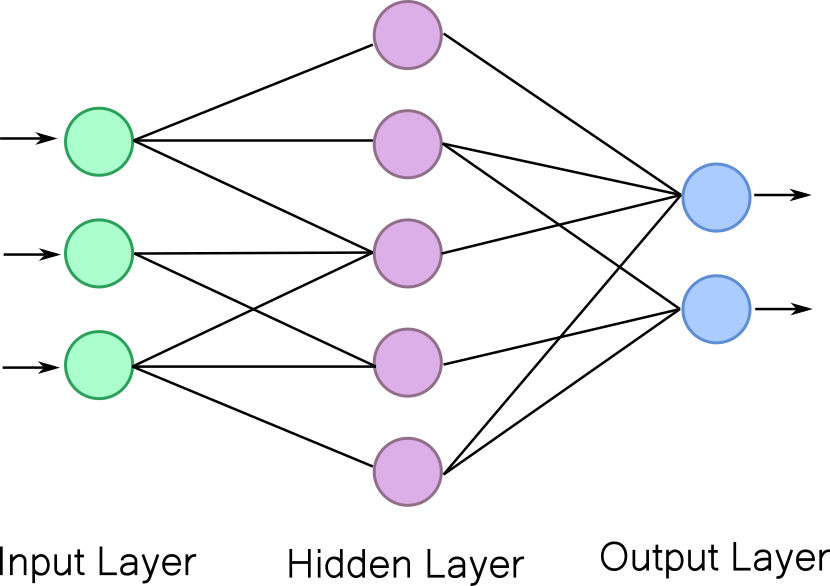
\includegraphics[width=0.6\linewidth]{ffnn}
    	\caption{Abstract structure of a feed-forward neural network. A real network will have many more layers and a lot more neurons per layer. Own figure.}
    	\label{fig:ffnn}
    \end{minipage}
	\centering
	\hspace{5mm}
	\begin{minipage}[t]{0.45\textwidth}
		\centering
		\begin{tikzpicture}[scale=0.5, transform shape]
  			\begin{axis}[scale only axis,
    					axis lines=middle,
    					inner axis line style={=>},
    					xlabel={},
    					ylabel={},
    					ytick={-1,-0.5,...,1},
    					xtick={-1,-0.5,...,1},
    					ymin=-1,
    					ymax=1,
    					xmin=-1,
    					xmax=1
  						] 
    			\addplot [mark=none,  blue,   ultra thick] {max(0, x)}; 
  			\end{axis}
		\end{tikzpicture}
    	\caption{Visualization of the ReLU activation function. Own figure.}
    	\label{fig:relu}
    \end{minipage}
\end{figure} 

\section{Neural Networks}

In the last couple of years neural networks and especially deep learning have gained more and more interest. The following sections dissect the individual components of a neural network and explain concepts and procedures.

\subsection{Neuron}

A \textit{Neuron} is the smallest unit of a neural network, this is what the network is build of. It essentially computes the linear function 

\begin{align}
y = \sum\limits_{i=0}^kw_ix_i + b
\end{align}

where $w_i$ is the weight for the $i$-th input $x_i$ and $b$ is a bias. The weights and the bias are the values that can be learned during the training process of the network (see section \ref{section:network_training}). The output of a layer of neurons of a network is the vector $(y_0, \cdots, y_t)$, $y_j$ being the output of the $j$-th neuron. Those outputs then serve as inputs to the next layer, although not every output has to be used by every next neuron. To prevent the network from collapsing into a single linear classifier and thus to increase the expressivity of the network, the output of a neuron is put into a non-linear so-called activation function. Although many different activation functions exist, most popular is the one called \textit{Rectified Linear Unit (ReLU)}, which was first presented by Jarrett et al. in \cite{relu}. The function is exemplarily visualized in fig. \ref{fig:relu} and is calculated as

\begin{align}
f(x) = max(0, x)
\end{align} 

\subsection{Feed-Forward Neural Network}

A \textit{Feed-Forward Neural Network} is a network consisting of layers of neurons. The first layer is called the input layer. Those are the neurons that actually receive the RGB values of an image for example. The last layer is called the output layer. The output of the neural network depends on the design implied by the use case. It can be class probabilities for classification tasks or object coordinates in our case. The intermediate layers are called hidden layers. Their number can grow to over a hundred in modern networks \cite{resnet}, thus the name deep neural networks and deep learning. All layers can have different numbers of neurons and connections to previous layers. A schematic overview over the structure of a neural network can be seen in fig. \ref{fig:ffnn}. 

\subsection{Convolutional Neural Networks}

\textit{Convolutional Neural Network} describes a certain type of feed-forward neural network that consists of mainly two types of layers.

\subsection{Network training} \label{section:network_training}

When a network is created, usually its weights and biases are initialized to 0 or sampled randomly from a Gaussian distribution. %TODO: cite
But this means, that the networks output is 

% Error back-propagation
% Gradient Descent
	% SGD
	% ADAM

\section{6D Pose Estimation}

\begin{figure}[!tbp]
	\centering
	\begin{subfigure}[t]{0.3\textwidth}
		\centering
    	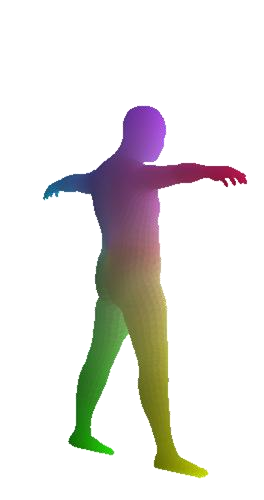
\includegraphics[width=0.45\linewidth]{human_object_coordinates}
    	\caption{The object coordinate representation of a human  \cite{tsharp}.}
    	\label{fig:human_object_coordinates}
	\end{subfigure}
	\begin{subfigure}[t]{0.3\textwidth}
		\centering
    	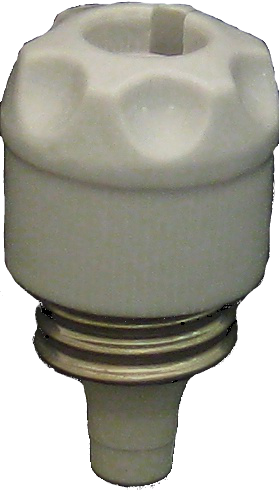
\includegraphics[width=0.45\linewidth]{tless_object}
    	\caption{An example object from the T-Less dataset \cite{tless}.}
    	\label{fig:tless_object}
	\end{subfigure}
	\begin{subfigure}[t]{0.3\textwidth}
		\centering
    	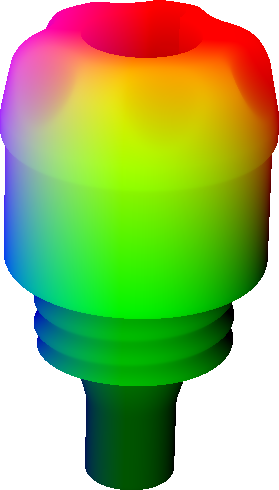
\includegraphics[width=0.45\linewidth]{tless_object_coordinates}
    	\caption{And the corresponding rendered 3D object coordinates (scaled for visualization). Own figure.}
    	\label{fig:tless_object_coordinates}
	\end{subfigure}
	\caption{Example 3D coordinate representations.}
\end{figure} 

\textit{6D pose estimation} is a central task in the computer vision community. The goal is to retrieve an object's translation and rotation from an image, relative to the camera. \textit{6}D refers to the \textit{6-Degrees-of-Freedom (6-DOF)}, i.e. the 6 free parameters of the \textit{3}D translation and \textit{3}D rotation. The field of application ranges from medical imaging, like in our case, robotics, augmented reality, and many others. 

Different systems provide different accuracy. Setups using two cameras for stereo vision or depth information in addition to colors achieve good results. As endoscopes usually do not provide depth information or stereo vision, this work focuses on pose estimation using RGB-only images. 

Early approaches extracted sparse features from the image and matched them against a large database to retrieve the pose. The accuracy of those methods suffers when objects are texture-less or poor-textured. Template-based methods rely mainly on the object's shape and therefore still work well on texture-less objects. Unfortunately, deformation of the object or partial occlusion is not handled well by templates and accuracy decreases significantly.

Deep learning enabled researchers to avoid manually modelling the features that are to be matched and instead make the systems learn the objects' appearances. There are different possible ways to estimate the pose with learning-based approaches. The 6 parameters can be predicted directly or an intermediate representation can be used for pose computation. Predicting the parameters directly can be problematic, as the output of the neural network underlies noise and there is no possibility to verify or improve the pose afterwards. This is the reason why this work employs a network with a dense output, i.e. one output (not one pose!) for each pixel. Each subset of pixels "votes" for a certain pose. Some pixels may contradict a pose and the pose with the least contradictions wins. The output for a pixel are the 3D coordinates on the object. The next section will introduce this concept of so-called object coordinates in depth.

\subsection{Object Coordinate Regression} \label{objectcoordinates}

Tayler et al. first used object coordinates in \cite{tsharp}. Instead of directly predicting the location of joints or limbs of the human body they computed the corresponding 3D location for each pixel of the image on the person (see fig. \ref{fig:human_object_coordinates}). The idea can be transfered to objects of any kind. Fig. \ref{fig:tless_object} shows an example object from the T-Less dataset \cite{tless} and fig. \ref{fig:tless_object_coordinates} shows the corresponding rendered 3D object coordinates.

The 3D coordinates and the respective 2D locations on the image imply the \textit{Perspective-n-Point (PnP) Problem}. That is, for a 2D point $u$ on the image and the corresponding 3D point $p$ (both in homogeneous coordinates), a pose consisting of the rotation matrix $R$ and the translation vector $t$ has to fullfil the following equation

\begin{align}
 u = K \ [ \ R \ | \ t \ ] \ p
\end{align} 

where $K$ is the camera matrix

\begin{align}
K = \begin{bmatrix}
f_x & s & c_x \\
0 & f_y & c_y \\
0 & 0 & 1 
\end{bmatrix}
\end{align}

which projects the 3D point transformed into the camera coordinate system on the 2D image plane. $s$ is a skew factor which is usually $0$, $(c_x, c_y)$ is the principal point, i.e. the center, of the image and $f_x$ and $f_y$ is the focal length in $x$ and $y$ direction respectively. The values for those variables can vary when the image was cropped or modified otherwise.

The relation is visualized in fig. \ref{fig:pnp}. Different solutions exists for variations of the problem. Gao et al. provide a method to solve it for exactly 3 2D-3D correspondences \cite{p3p}. But using only 3 points to compute the pose does not take into account all the information we obtain from the neural network and is more suitable for hand-picked correspondences. Using P3P, a possible scenario is that the automatic process picks three outlier correspondences and thus produces an incorrect pose. \textit{EPnP} \cite{epnp} is the algorithm by Lepetit et al. that solves the PnP problem for \textit{n} points.

\begin{figure}[!tbp]
	\centering
    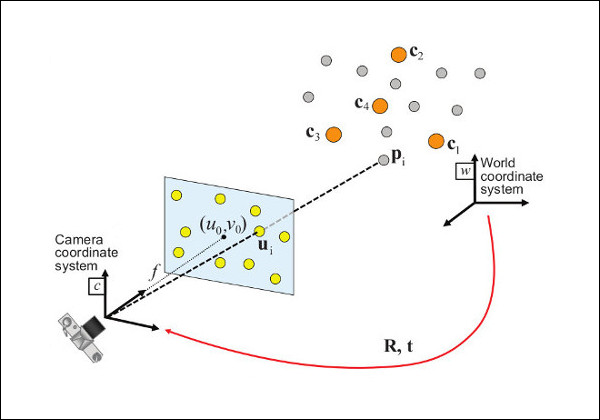
\includegraphics[width=0.45\linewidth]{pnp}
    \caption{The relationship between the camera, the 3D points and their projections on the screen using the rotation matrix $R$ and the translation vector $t$ \cite{opencv_pnp}.}
    	\label{fig:pnp}
\end{figure} 

Another common method to solve the PnP problem is to use the \textit{RANSAC algorithm} \cite{ransac} or a variation of it. Since RANSAC is well known and employed in many different applications to estimate a model that fits a dataset best, we will use it in this work to establish mathematical relationship between the predicted 3D object coordinates and their 2D locations. 

The implementation that is used is the one incorporated into the \textit{solvePnPRansac} method of the \textit{OpenCV} \cite{opencv} framework. Algorithm \ref{algorithm:ransac} shows the outline of the RANSAC algorithm for pose estimation. The energy function can be varied. It can for example be the number of inliers, i.e. the number of 3D points whose difference of the reprojected 2D location and the actual 2D location is within a certain threshold.

\begin{algorithm}
\caption{RANSAC} \label{algorithm:ransac}
\begin{algorithmic} 
\REQUIRE Set of 3D points
\REQUIRE Set of corresponding 2D points
\REQUIRE Number of iterations $i$
\REQUIRE An energy function to score the pose hypothesis $E$
\STATE Set current energy $e=0$
\STATE Set current best pose hypothesis $h$ to $null$
\FOR{$1 ... i$}
\STATE Select a subset of corresponding points to compute pose $H$
\STATE Compute energy of the pose $e'=E(H)$
\IF{$e' > e$}
\STATE Store pose $H$ as current best in $h$
\STATE Set $e = e'$
\ENDIF
\ENDFOR
\RETURN Best pose $h$
\end{algorithmic}
\end{algorithm}